\chapter[Solutions: Chapter \ref{cedc0}]
        {Solutions: Chapter \ref{cedc0}, \cedczerolongtitle{}}

\label{ceds0}

\vworkexercisechapterheader{}

%%%%%%%%%%%%%%%%%%%%%%%%%%%%%%%%%%%%%%%%%%%%%%%%%%%%%%%%%%%%%%%%%%%%%%%%%%
%%%%%%%%%%%%%%%%%%%%%%%%%%%%%%%%%%%%%%%%%%%%%%%%%%%%%%%%%%%%%%%%%%%%%%%%%%
%%%%%%%%%%%%%%%%%%%%%%%%%%%%%%%%%%%%%%%%%%%%%%%%%%%%%%%%%%%%%%%%%%%%%%%%%%

\begin{vworkexercisesolution}{\ref{exe:cedc0:sexe0:01}}

\begin{figure}
\centering
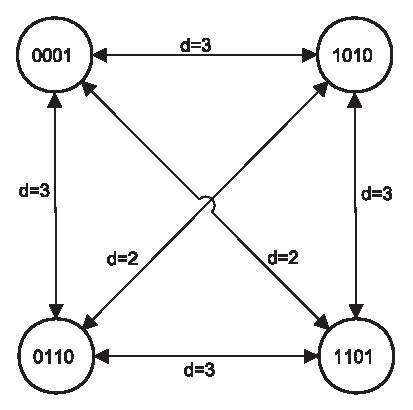
\includegraphics[height=3.0in]{c_eds0/exe001.eps}
\caption{Graphical Solution To Exercise \ref{exe:cedc0:sexe0:01}}
\label{fig:ceds0:exe01:01}
\end{figure}

The relationships between the four codewords of this code can be
depicted as in Figure \ref{fig:ceds0:exe01:01}.  For example,
the Hamming distance between 0001 and 1010 is 3, and the
Hamming distance between 0110 and 1010 is 2.

Since the minimum Hamming distance $\hat{d}$ is defined as the minimum
Hamming distance between any two codewords, this distance is 2.

\end{vworkexercisesolution}

%%%%%%%%%%%%%%%%%%%%%%%%%%%%%%%%%%%%%%%%%%%%%%%%%%%%%%%%%%%%%%%%%%%%%%%%%%
%%%%%%%%%%%%%%%%%%%%%%%%%%%%%%%%%%%%%%%%%%%%%%%%%%%%%%%%%%%%%%%%%%%%%%%%%%
%%%%%%%%%%%%%%%%%%%%%%%%%%%%%%%%%%%%%%%%%%%%%%%%%%%%%%%%%%%%%%%%%%%%%%%%%%


%\vworkexerciseseparator
%\begin{vworkexercisesolution}{\ref{exe:cedc0:sexe0:01}}
%Placeholder.
%\end{vworkexercisesolution}
\vworkexercisechapterfooter

%End of file c_eds0.tex

